\documentclass{class}

%-----------------------------------------------------------------
\titleind{Tugas}

\fullname{Afrizal Dani Saoqi}

\idnum{17/413500/TK/45940}

\papername {Perancangan Sistem Digital}

\degree{Teknik Elektro}

\yearsubmit{2020}

\program{Teknik Elektro}

\dept{Teknik Elektro dan Teknologi Informasi}


%-----------------------------------------------------------------



\usepackage[titles]{tocloft}
\renewcommand\cftfigpresnum{Gambar\  }
\renewcommand\cfttabpresnum{Tabel\   }

%Untuk hyperlink dan table of content
\usepackage{hyperref}
\newlength{\mylenf}
\settowidth{\mylenf}{\cftfigpresnum}
\setlength{\cftfignumwidth}{\dimexpr\mylenf+2em}
\setlength{\cfttabnumwidth}{\dimexpr\mylenf+2em}

%Untuk Bold Face pada Keterangan Gambar
\usepackage[labelfont=bf]{caption}

%Untuk caption dan subcaption
\usepackage{caption}
\usepackage{subcaption}
\usepackage{listings}
\usepackage{rotating}
\begin{document}
\cover
\section{Decoder 2 to 4 using behavioral modeling}
    \begin{enumerate}
        \item Architecture
        \begin{figure}[H]
            \centering
            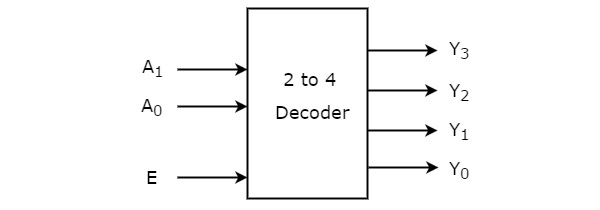
\includegraphics[width=1\linewidth]{gambar/2_to_4_decoder.jpg}
            \caption{Architecture}
            \label{Architecture}
            \end{figure}
        \item Source Code
        \lstinputlisting{code/24.v}        
        \item TestBench Source Code
        \lstinputlisting{code/tb_decoder_24.v}
        \item Command Line
        \begin{figure}[H]
            \centering
            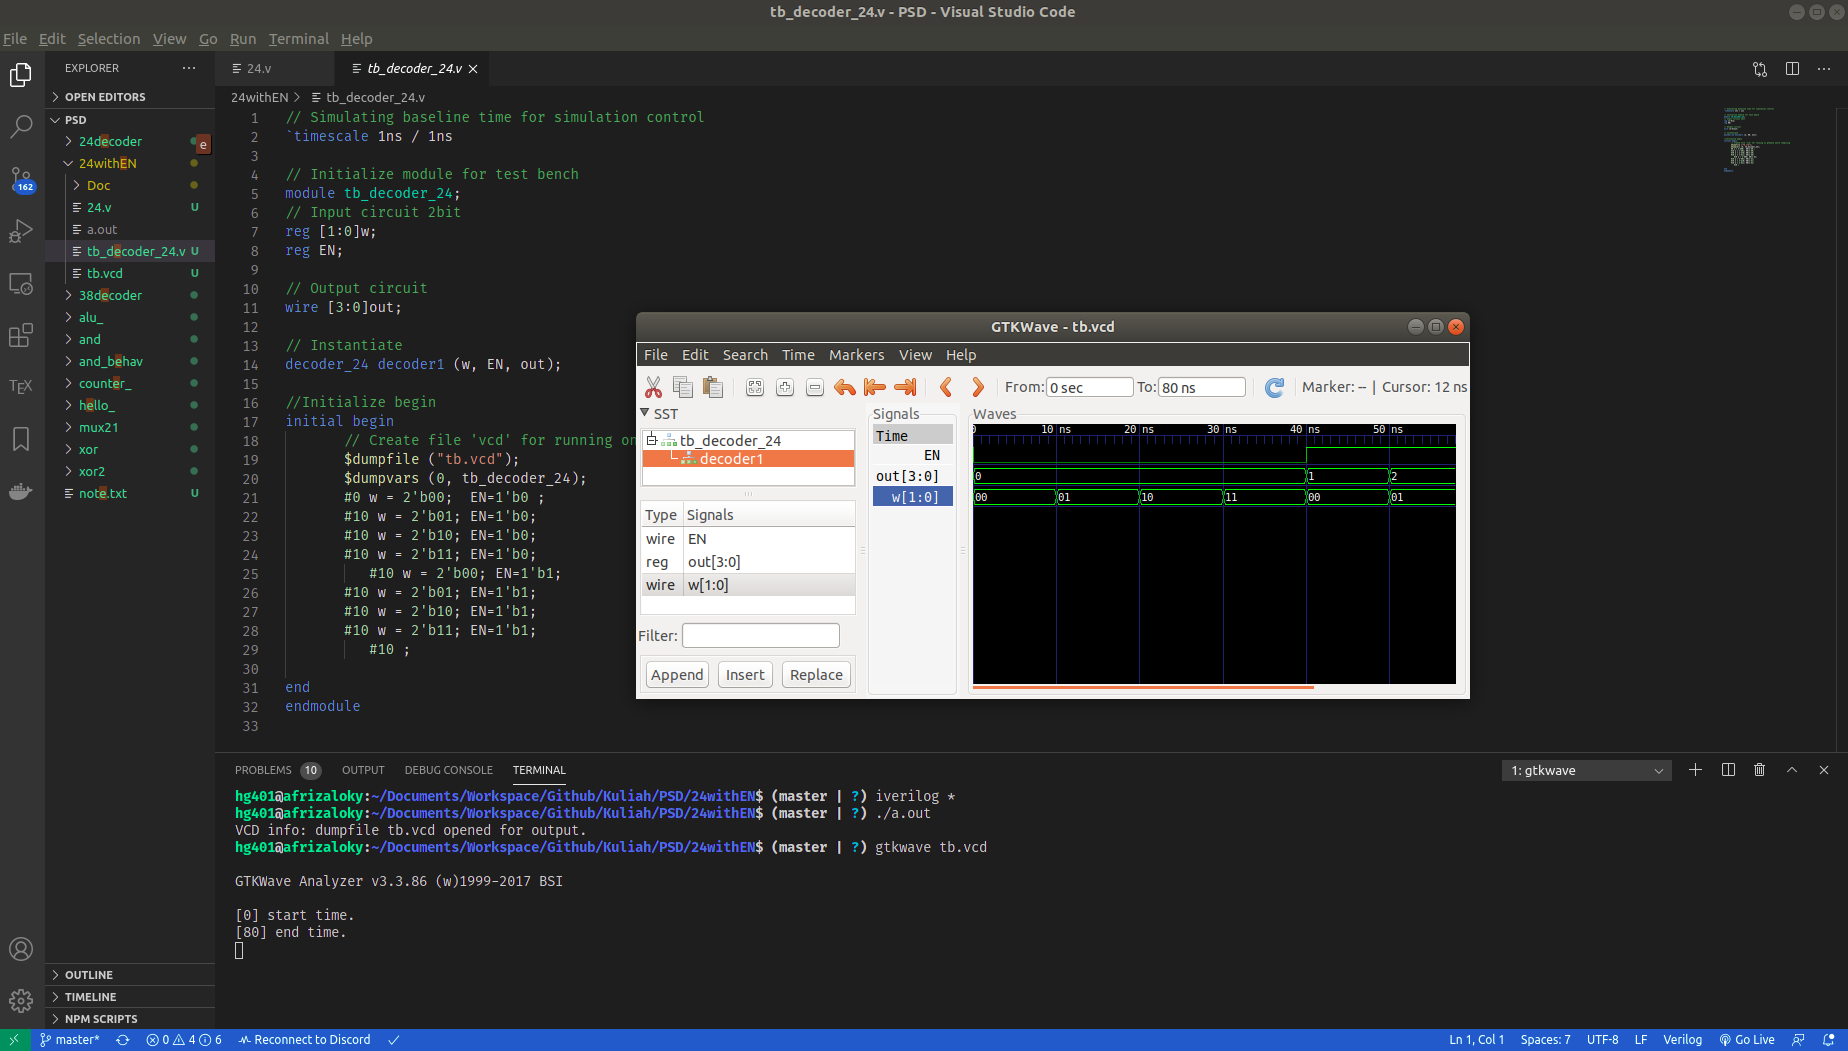
\includegraphics[width=1\linewidth]{gambar/cmd.png}
            \caption{Command Line}
            \label{cmd}
            \end{figure}
        \item Simulation
        \begin{figure}[H]
            \centering
            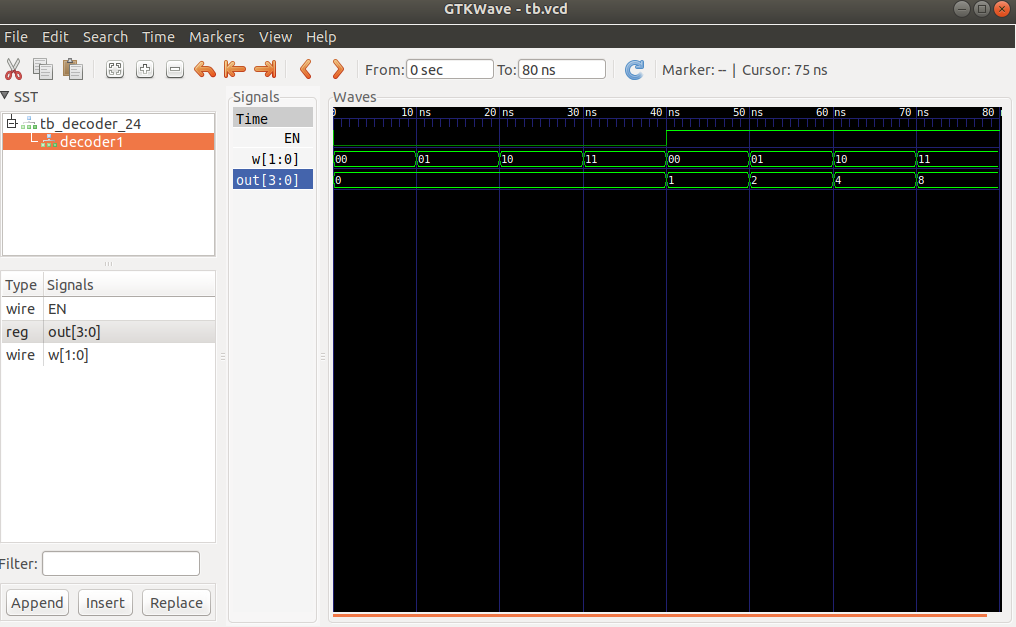
\includegraphics[width=1\linewidth]{gambar/simlasi_24.png}
            \caption{Simulasi Decoder 2 to 4}
            \label{decoder24}
            \end{figure}
    \end{enumerate}


\section{Decoder 3 to 8 using decoder 2 to 4}
\begin{enumerate}
    \item Architecture
    \begin{figure}[H]
        \centering
        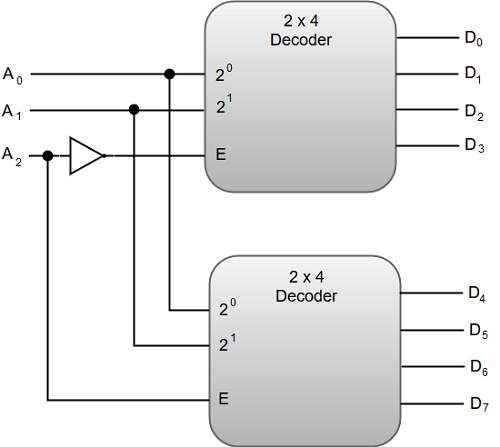
\includegraphics[width=1\linewidth]{gambar/decoders3.png}
        \caption{Architecture}
        \label{Architecture}
        \end{figure}
    \item Source Code 2 to 4
    \lstinputlisting{code/24.v}   
    \item Source Code 3 to 8 using 2 to 4
    \lstinputlisting{code/decoder_38.v}        
    \item TestBench Source Code
    \lstinputlisting{code/tb.v}
    \item Command Line
    \begin{figure}[H]
        \centering
        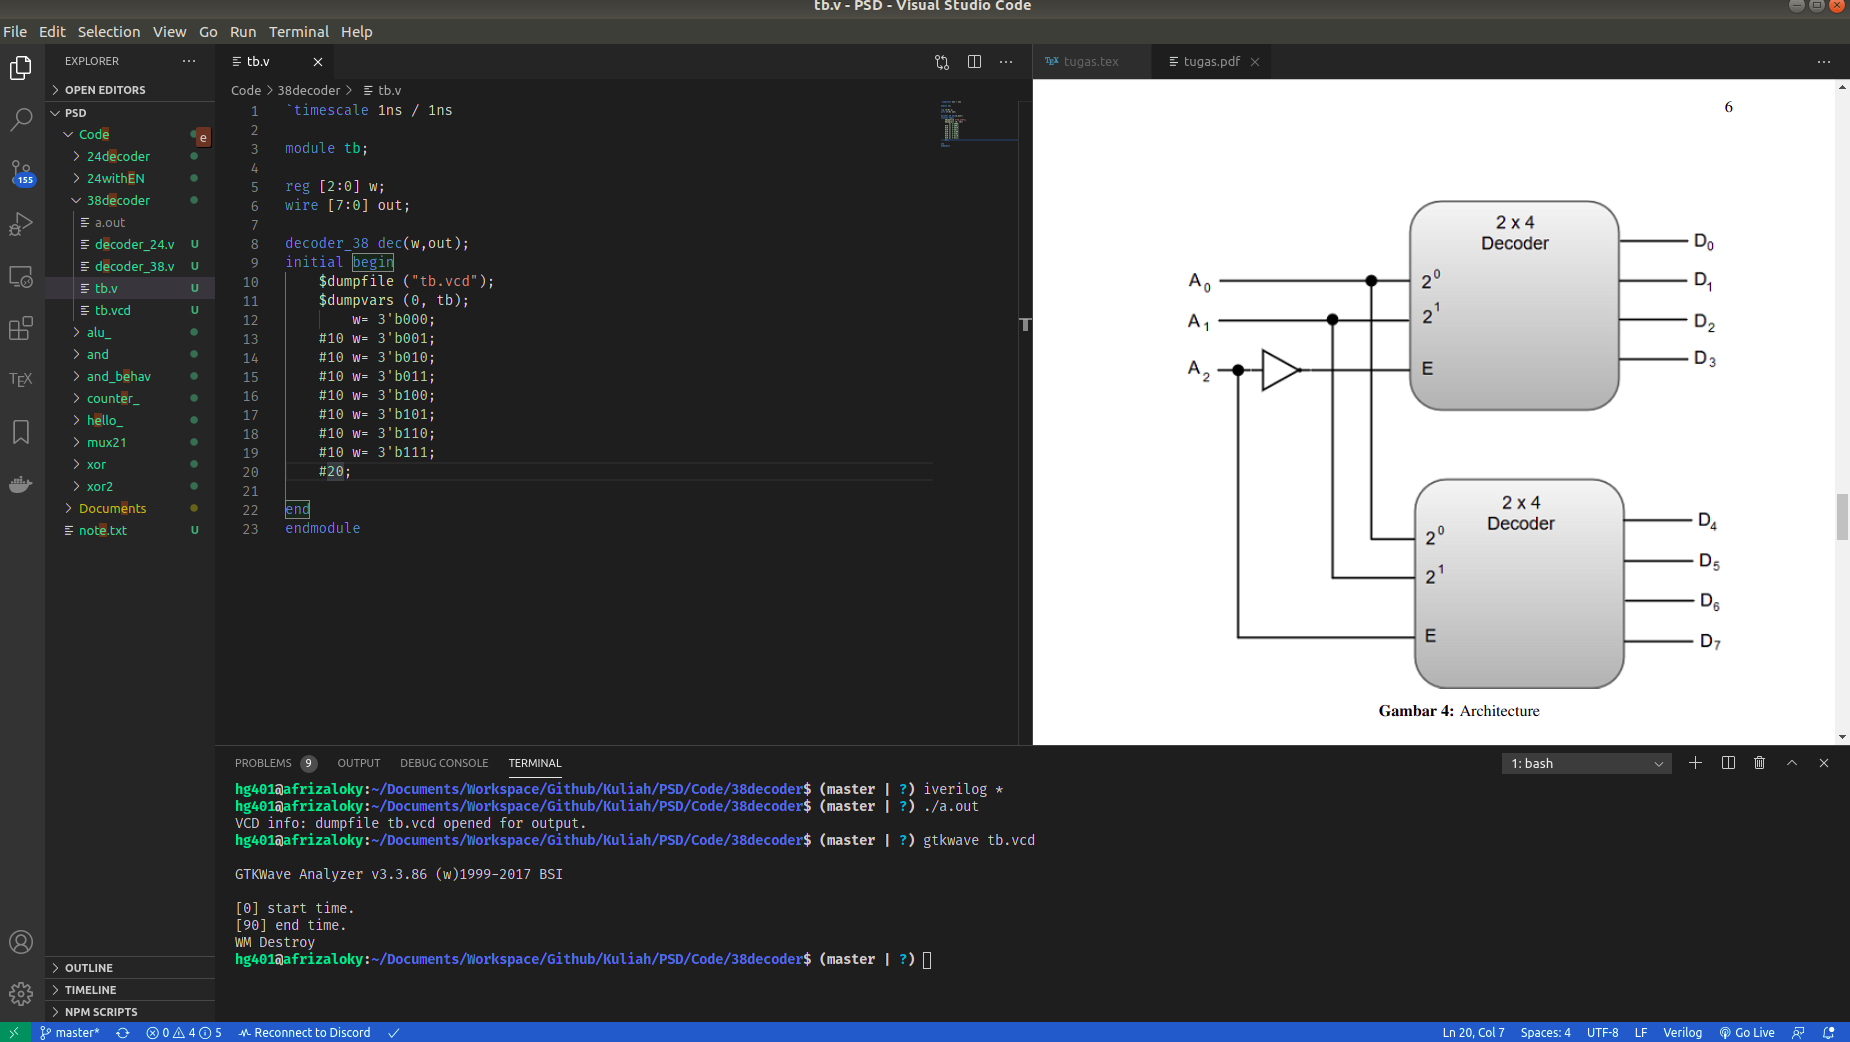
\includegraphics[width=1\linewidth]{gambar/cmd38.png}
        \caption{Command Line}
        \label{decoder24}
        \end{figure}
    \item Simulation
    \begin{figure}[H]
        \centering
        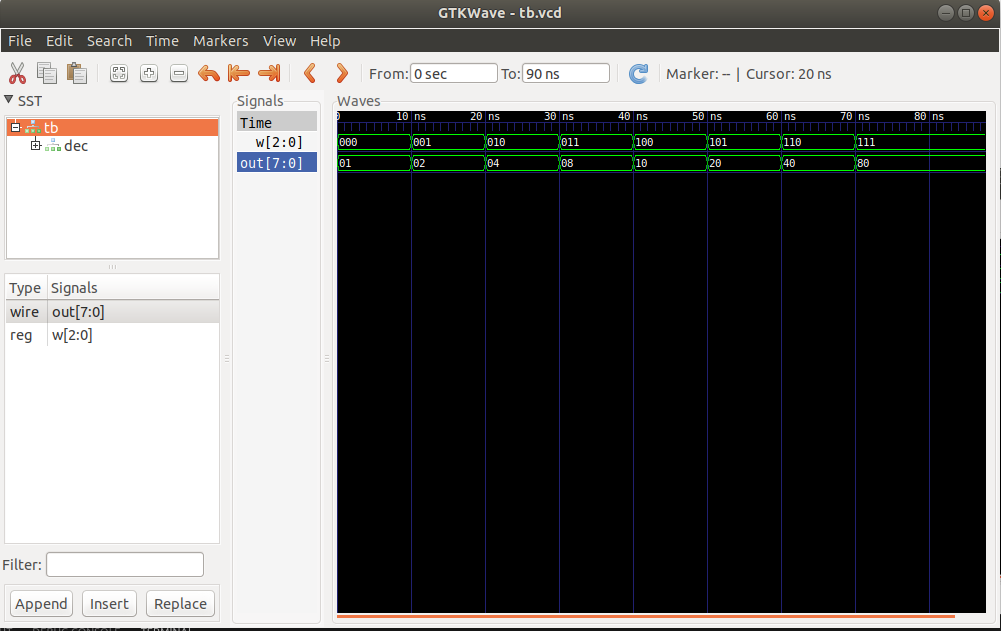
\includegraphics[width=1\linewidth]{gambar/simulation38.png}
        \caption{Simulasi Decoder 3 to 8}
        \label{decoder24}
        \end{figure}
\end{enumerate}
\end{document}